\chapter{Active Learning in Real-time Bidding (RTB)}
\label{chapterlabel4}

In this chapter, we discuss a dynamic programming process. It always happens since no advertiser knows the information from the market at the first time. For the purpose of maximising present utility, they may bid a price to test the market and actively learn from the feedbacks. This sacrifice may increase the utility in the future.

Some prior work focuses on the dynamic optimization of bidding strategy  \cite{christianborgsjenniferchayesomidetesaminicoleimmorlicakamaljainmohammadmahdian2007} gives a 
heuristic equilibria of biding optimization which can characterize the behavior of each advertiser in a repeated sponsored search auction. In those use cases, the problem is described as a form of the multi-armed bandits problem for efficiently allocating the ad slots and simultaneously estimating the CTR \cite{peterauernicolocesabianchipaulfischer2002}. Also, some researches apply dynamic programming to discovering the CTR of the ads. 

There is always a discount of payoffs in repeated auctions. The exploration process leads to an incentive exceeding true value to increase their bid by an amount which is called \emph{value of learning} \cite{saiminglimohammadmahdianr.prestonmcafee2010}. There are several papers that give explore-exploit algorithms for this problem in machine learning perspective \cite{deepakagarwalbeechungchenpradheepelango2009}. Typically, utility in auction environment can be approximated by Taylor expansion \cite{patrickhummelr.prestonmcafee2014}. 

The other practical problem is that the market price landscape is often uncertain. Markov decision process (MDP) is an expression which can be used to perform the repeated online decisions for censored data \cite{Amin_budgetoptimization, ivantajduharbojanadalbeloba2012}. In terms of right censored observations, Product-Limit algorithm is a computational way to fit the real price distribution \cite{e.l.kaplanpaulmeier1958}. Learning from unknown situation can be treated as an active learning process \cite{robertzeithammer2007}. Active learning is a special semi-supervised machine learning in which a method is able to interactively obtain the optimal sequential outcome \cite{burrsettles2010}.

Consider the following typical RTB auction: We have a fixed $N$ number of advertisers $i \in \{1,...,N\}$ with the same target rule. In other words, they will simultaneously see same impression requests hitting the target rule over a period of time and compete with each other to bid the impressions. The features from the bid request are denoted as a high-dimensional column vector $\mathbf{x}_t$, where $t \in \{1,...,T\}$. We use $\delta$ as the time discount. Each advertiser has their own assessment about the value of each impression based on $x_t$ and their business needs. Without loss of generality, let us assume that all the advertisers are focused on direct response from end users with clicks. In other words, the value of the impression is CTR for their own campaigns. And let us assume a symmetric situation where each advertiser has the same valuation of the click (Cost Per Click), which is set to 1. Each of them employs a logistic regression to estimate the probability of click given $\mathbf{x}_t$, i.e., 
\begin{align}
\label{eq:logistic_regressor}
\theta_i \equiv p(c=1|\mathbf{x}_t;\mathbf{w}_i) \equiv \sigma(\mathbf{w}_{i}^{T}\mathbf{x}_t) = \frac{1}{1+\exp{(-\mathbf{w}_{i}^{T}\mathbf{x}_t})}
\end{align}
where the CTR estimation is through a linear combination of model parameters $\mathbf{w}_i$ and $\mathbf{x}_t$ with a transformation function. The $\mathbf{w}_i$ follows a Gaussian prior $\mathcal{N}(0, \alpha ^{-1}\bs{I})$, where is a diagonal matrix. $\theta_i$ denotes the true value of the auction $t$. The true value is bounded between $[0,1]$ and its estimation is through a linear combination of model parameters $\mathbf{w}_i$ and $\mathbf{x}_t$. Again, we assume the $\mathbf{w}_i$ follows a Gaussian prior $\mathcal{N}(0, \alpha ^{-1}\bs{I})$, where is a diagonal matrix. 

Our problem is for each advertiser what is the optimal bid the following different settings: 

\begin{enumerate}

 \item A simplest situation is that $t=1$ and each advertiser knows their own CTR and thus $\mathbf{w}_i$. We need to show in this setting, the optimal bid $b_i$ for advertiser $i$ is $b(\mathbf{x}_1;\mathbf{w}_i)$ = $p(c=1|\mathbf{x}_1;\mathbf{w}_i)$.

 \item A slightly more complicated case is that the auction repeated running finitely from $t=\{1,...,T\}$. $\mathbf{x}_t\sim \mathcal{N}(0,\gamma \bs^{-1}\bs{I})$. In this case, each advertiser $i$ still knows their $\mathbf{w}_i$. What is the optimal $b(\mathbf{x}_t; \mathbf{w}_i,\alpha,\gamma ,\sigma)$?

Are we getting the same result as in the previous case or something different? In this case, as each advertiser knows their value so no information exploration for true value, but they can have an exploration on the market price landscape. Intuitively, we should get a higher bid than the previous case or we would obtain the same conclusion? 

\end{enumerate}


\section{One-shot RTB Auction}

In one-shot game, there is only one impression in total, namely $t \in \left \{ 1 \right \}$. In terms of a second price auction, we suppose ad $i$'s true value is the CTR
\begin{equation}
\theta_i\equiv p(c=1|\mathbf{x}_1;\mathbf{w}_i)
\end{equation}

We assume the game has a Bayesian Nash equilibrium bidding strategy. If the advertiser $i$ believes bidding price $b_i>\theta_i$. Given $\theta_t$ denotes the highest bid of the other bidders $j$ where $j\neq i$. Advertiser $i$ has no information about advertiser $j$ before the one-shot bidding begins. Thus, from $i$'s perspective, the bid of $j$ is treated as a random variable. Here, we have three potential results for the one-shot game. They are (i) $\theta_t>b_i,\theta_i$; (ii) $b_i>\theta_t>\theta_i$; or (iii) $b_i,\theta_i>\theta_t$ respectively. Considering the first and the third outcome, since the belief is $b_i>\theta_i$, advertiser $i$ will bid $\theta_i$ instead of bidding $b_i$ in the rational situation. In (i), no chance to win indicates that he will not pay anything. In (ii), he can win the bid but pay more than the true value $\theta_i$, which does not follow the auction assumption, so case (ii) will not happen. In (iii), bidding the true value $\theta_i$ can win the bid. Therefore, the optimal bidding strategy for ad $i$ is to bid the true value when $b_i>\theta_i$. Likewise, we also can prove if his belief turns to be $b_i<\theta_i$, the optimal bidding price is still equal to the true value $\theta_i$.

In summary, for a second price bid, each bidder will bid their true value in one-shot game as their optimal bidding strategy:
\begin{equation}
\label{eq:bidding true value}
b_{i}^{*}=\theta_i
\end{equation}
which can maximize the utility. Once advertiser $i$ wins the impression, he will be charged for $\theta_t$ in the second price auction.

\section{Sequential Auction with Certain CTR}

In a repeated game, at any time step $t$ where $t\in \left \{ 1,2,...,T\right \}$, namely there are infinite impressions that advertisers can bid, the state $s$ can be described as two numbers $s\in \left \{(n,t)  \right \}$, giving a state where the ads of the advertiser has been shown $t$ times and out of these impressions, $n$ of them have lead to winning. let $b_i$ denote the bid of the advertiser $i$ and $\theta_{i}$ denote the expected clickability at this state. If $\theta_t<b_{i}$, then the advertiser wins the bidding and has to pay $\theta_t$. We assume a discount factor of $\delta<1$ for calculating present utility. As the CTR $\theta_i$ of ad $i$ is certain, the known $\mathbf{w}_i$  incorporates all the information that can be learned from winning bid request $\mathbf{x}_t\sim \mathcal{N}(0,\gamma \bs^{-1}\bs{I})$. In this case, as each advertiser knows their value so no information exploration. Let us assume we do not update belief about other advertiser's CTR estimation. Thus, the utility in one round can be expressed as
\begin{equation}
u(b_i,\theta_i)=E[(\theta_i-\theta_t)\bm{I}_{b_i>\theta_t}]
\end{equation}
The probability of $\theta_t$ follows pdf and cdf are $f(\cdot)$ and $F(\cdot)$ respectively, which can be interpreted as market price distribution. It is the highest valuation among other $N-1$ players in the campaign. The above expression at time $t$ can be rewritten as
\begin{equation}
\label{eq:utility}
u(b_i,\theta_i)=\int_{0}^{b_i}(N-1)(\theta_i-\theta_t)f_{n}(\theta_t)F_{n}(\theta_t)^{N-2}d\theta_t
\end{equation}
Since $\theta_t \in [0,1]$, define 
\begin{equation}
f_{n}(\cdot) \leftarrow (N-1)f_{n}(\cdot)F_{n}(\cdot)^{N-2}
\end{equation}
and then the Eq.~(\ref{eq:utility}) can be expressed as
\begin{equation}
\label{eq:utility}
u(b_i,\theta_i) = \int_{0}^{b_i}(\theta_i-\theta_t)f_{n}(\theta_t)d\theta_t
\end{equation}
In this scenario \cite{menezes2005introduction} , we assume that no update is needed when losing the bid. If the advertiser $i$ win the bid, he can obtain the information of market price, which can be used to update the estimation of market price landscape. The workflow of the active learning is shown in Figure~\ref{fig:active}. 

\begin{figure}[htbp]
\centering
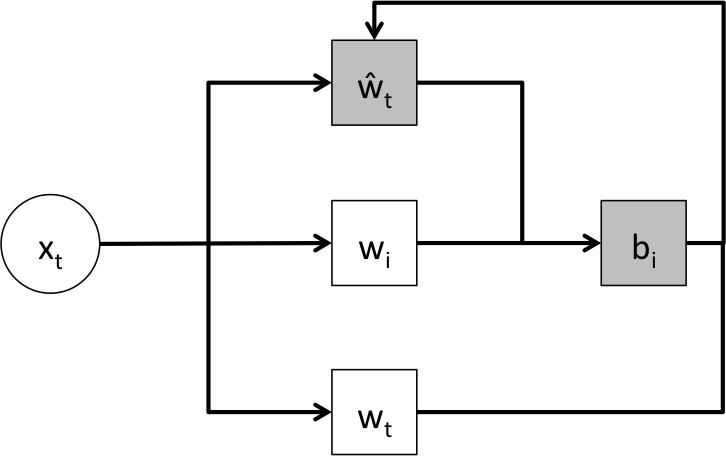
\includegraphics[width=0.6\textwidth]{active.png}
\caption{The workflow chart of active learning in sequential auction with certain CTR}
\label{fig:active}
\end{figure}
Besides, the observation of clickability will not have any contribution to advertiser $i$ because his CTR is known and certain. Thus, the next status only has two situations, namely winning or losing the bid. The MDP is given by Figure~\ref{fig:MDPs}.
\begin{figure}[htbp]
\centering
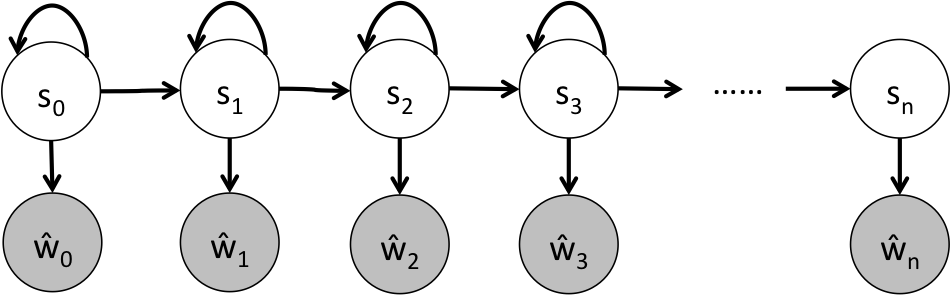
\includegraphics[width=0.8\textwidth]{MDPs.png}
\caption{Markov Decision Process (MDP) for the estimator of market price landscape}
\label{fig:MDPs}
\end{figure}

The total utility in the repeated auction can be simplified as 
\begin{equation}
\begin{split}
U(n,t)=\underset{b_{i}}{\max}\{ & u(b_i,\theta_i) + \delta F_{n}(b_i)U(n+1,t+1) \\
& + \delta (1-F_{n}(b_i))U(n,t+1) \}
\end{split}
\end{equation}
If advertiser $i$ wins the impression $n$, the market price distribution will update from $f_n$ to $f_{n+1}$. Otherwise it stays as $f_n$. Further, the above expression can be rewritten as
\begin{equation}
\label{eq:total utility}
\begin{split}
U(n,t)=\frac{1}{1-\delta}\underset{b_{i}}{\max}&\{ u(b_i,\theta_i)+\delta F_{n}(b_i) \\
& (U(n+1,t+1)-U(n,t+1)) \}
\end{split}
\end{equation}
Intuitively, assume bidding strategy $b_i$ is very small. $F_{n}(b_i)$ will be close to zero. If the second term is small enough that can be neglected, the remaining term is almost equivalent to a one-shot game. The optimal bidding price does not follow the assumption that $b_i$ is very small. On the other hand, assume bidding strategy $b_i$ is very large because we do not consider budget constraints here. $u(b_i,\theta_i)$ will turn to be negative while $F_{n}(b_i)$ increases. 

We can easily prove the bidding price for two-steps game is not equal to true value when achieving the maximum of total utility. Hence, in terms of short-term repeated games, the optimal biding strategy is not bidding true value.

\section{Greedy Product-Limit Algorithm}
In the previous section, we discuss how to find the optimal bidding strategy when $\theta_i$ is known. Now, we will discuss how we can update the market price distribution from $f_n$ to $f_{n+1}$ with the side information. Based on the setting above, winning an impression does not represent winning a click.

Suppose that $\mathcal{P}$ is a distribution with mass function $p$ and $(\theta_1,...,\theta_T)$ are i.i.d. random variables following $\mathcal{P}$-distribution. Fix $T$ integers $k_1,...k_T$, and define $o_t=\min (\theta_t,k_t)$. We say that sample $\{ o_t \}$ is partially right-censored data. Here, $k_t$ is equivalent to the bidding price $b_i$ for impression $t$.

If $o_t<k_t$, $o_t$ is a direct observation. The true value can be observed as $\theta_t$. Otherwise, $o_i$ is a censored observation. The only information is known as $\theta_t \geq k_t$. Given such partially right-censored data, the Product-Limit estimator is the non-parametric maximum-likelihood estimator for $p$.

Let $PL(K,O)$ be the Product-Limit estimator for $p$. Specifically, given integers $K$, and a set of observations $O$ generated by a distribution $\mathcal{P}$, let $D(s)=|\{o_t \in O|s=o_t<k_t\}|$ be the number of direct observations of value $s$, and $N(s)=|\{o_t \in O|s \leq o_t,s<k_t\}|$. Now, let 
\begin{equation}
\label{eq:PL}
S(t)=\prod_{s=1}^{t-1}{1-\frac{D(s)}{N(s)}}
\end{equation}
Hence, the CDF of $PL(K,O)$ is given by $1-S(t)$. 

The market price distribution $\mathcal{P}$ will be updated after certain number of bids using Greedy Product-Limit Algorithm \cite{Amin_budgetoptimization}.

\section{Temporal Difference (TD) Learning for Optimal Bidding}

\subsection{Q-Learning: Off-Policy TD Control}

For the second case, we take the derivative of the expression in Eq.~(\ref{eq:total utility}) to compute the optimal bid
\begin{equation}
\frac{{\partial U(n,t)}}{{\partial {b_i}}} = ({\theta _i} - {b_i})f({b_i}) + \delta f({b_i})(U(n + 1,t + 1) - U(n,t + 1))
\end{equation}
Let this equal zero. Hence, the optimal bid of the advertiser $i$ can be written as
\begin{equation}
{b_{i}^{*}} = \theta_i + \delta (U(n+1,t+1)-U(n,t+1))
\end{equation}
After receiving enough information from the market, it leads to $f_{n+1}\approx f_{n}$, which means $(U(n+1,t+1)-U(n,t+1))\approx 0$. Hence, in the very long-term after learning market price landscape is converged, maximizing total utility is equivalent to find a optimal bidding price for a one-shot game if the market environment is steady.

Since the above is equivalent to a dynamic programming problem. That is, starting from state $s(0)=s$ at impression $t=0$. Each state contains two elements: number of winning bids $n$ and number of total bidded impressions $t$. It should choose action $a(0),a(1),...,a(T)$ which is the bidding price to maximize the expected long term rewards available starting from $s$ and following policy $\pi$. Here, the reward is the utility that the advertiser may have. The given MDP formulation is
\begin{equation}
U^{*}(s)=\underset{\pi}\max U^{\pi}(s)=\underset{a} \max \left \langle \sum_{t=0}^{\infty }\delta^{t}u(s(t),a(t)) \right \rangle_{s,u}
\end{equation}
At any impression $t$, we can rewrite the optimization problem as a recursive expression
\begin{equation}
U^{*}(s(t))=\underset{a(t)} \max E_{s(t+1)}[u(s(t),a(t),s(t+1))+\delta U^{*}(s(t+1))]
\end{equation}
The optimal function is a Bellman equation.
Let
\begin{equation}
U^{\pi}(s)=\underset{a} \max Q^{\pi}(s,a)
\end{equation}
The utility equation will transform to be
\begin{equation}
\begin{split}
Q^{*}(s(t),a(t)) & =E_{s(t+1)}[u(s(t),a(t),s(t+1)) \\
& +\delta \underset{a(t+1)} \max Q^{*}(s(t+1),a(t+1))]
\end{split}
\end{equation}

Since advertisers do not know the expected rewards and the transition matrices, we can use Q-Learning to solve the Bellman equation \cite{michaelgabrieljohnmoore1991, richards.suttonandrewg.barto1998}. Assume state $s(t) \in \left \{(n,t)  \right \}$ and $s(t+1)\in \left \{(n,t+1),(n+1,t+1)  \right \}$. In the next state, the bided impression will increase 1 and there will be two results for the advertiser, winning or losing the impression. 

The overall update at time $t$ is
\begin{equation}
\label{eq:QlearningQvalue}
\begin{split}
Q(s(t),a(t)) \leftarrow & Q(s(t),a(t)) +\epsilon [u(s(t),a(t),s(t+1)) \\
&+\delta \underset{a(t+1)}\max Q(s(t+1),a(t+1))-Q(s(t),a(t))]
\end{split}
\end{equation}
where $u(s(t),a(t),s(t+1))=u(b_i,\theta_i)$ in Eq.~(\ref{eq:utility}). As in value iteration, a policy of advertiser $i$ can be defined at any time according to 
\begin{equation}
\label{eq:optimalbid}
b^{*}_{i}=\underset{a(t)}\argmax Q(s(t),a(t))
\end{equation}
Also, we can use another temporal differences which is called Actor-critic learning which is a policy iteration approach. Q-Learning learns the optimal policy even when actions are selected according to a more exploratory or even random policy. As we use $\epsilon$-Greedy in Q-Learning, it encourages exploration as well.
\begin{algorithm}
\caption{Q-learning in repeated auctions with side information}
\label{al:Qlearning}
\begin{algorithmic}[1]
\Procedure{Q-Learning} {}
\\Initialize $Q(s,a)$ arbitrarily
\For{each episode}
\\ \qquad Initialize $s$
\For{each step of episode}
\\ \qquad \qquad Choose $a(t)$ from $s(t)$ using policy derived from $Q$ (e.g. $\epsilon$-Greedy) 
\\ \qquad \qquad Take action $a(t)$, observe $u$ and $s(t+1)$
\\ \qquad \qquad Update Q table using Eq.~\ref{eq:QlearningQvalue}
\EndFor
\EndFor
\EndProcedure
\end{algorithmic}
\end{algorithm}

\subsection{Sarsa: On-Policy TD Control}
The Sarsa algorithm is an On-Policy algorithm for TD-Learning. The major difference between it and Q-Learning, is that the maximum reward for the next state is not necessarily used for updating the Q-values. Instead, a new action, and therefore reward, is selected using the same policy that determined the original action.Sarsa and Q-Learning has the same Q update process, but the execution step is different. 

The utility equation will transform to be
\begin{equation}
\begin{split}
Q^{*}(s(t),a(t)) & =E_{s(t+1)}[u(s(t),a(t),s(t+1)) \\
& +\delta Q^{*}(s(t+1),a(t+1))]
\end{split}
\end{equation}

The overall update at time $t$ is
\begin{equation}
\label{eq:SarsaQvalue}
\begin{split}
Q(s(t),a(t)) \leftarrow & Q(s(t),a(t)) +\epsilon [u(s(t),a(t),s(t+1)) \\
&+\delta Q(s(t+1),a(t+1))-Q(s(t),a(t))]
\end{split}
\end{equation}

There are two action selection steps needed, for determining the next state-action pair along with the first. The parameters $\epsilon$ and $\delta$ have the same meaning as they do in Q-Learning.
\begin{algorithm}
\caption{Sarsa in repeated auctions with side information}
\label{al:Sarsa}
\begin{algorithmic}[1]
\Procedure{Sarsa} {}
\\Initialize $Q(s,a)$ arbitrarily
\For{each episode}
\\ \qquad Initialize $s$
\\ \qquad Choose $a(t)$ from $s(t)$ using policy derived from $Q$
\For{each step of episode}
\\ \qquad \qquad Take action $a(t)$, observe $u$ and $s(t+1)$
\\ \qquad \qquad Choose $a(t+1)$ from $s(t+1)$ using policy derived from $Q$
\\ \qquad \qquad Update Q table using Eq.~\ref{eq:SarsaQvalue}
\EndFor
\EndFor
\EndProcedure
\end{algorithmic}
\end{algorithm}

The optimal bidding strategy can be obtained from Eq.~\ref{eq:optimalbid} as well.

\section{Kernelized Value Function Approximation}
Let us simplify the Bellman equation of total utility Eq.~\ref{eq:total utility} to
\begin{equation}
U^{*} = u + \delta PU^{*} 
\end{equation}
Where $PU$ denotes the present value of future utility. For the purpose of approximation, we try to minimise $E(w)$ which is the squared error with regularized term
\begin{equation}
E(w) = \frac{1}{2} \sum_{i=1}^{N}(w^{T}\phi(x_i)-y_i)^{2}+\frac{\lambda}{2}w^{T}w
\end{equation}
Let 
\begin{equation}
\frac{{\partial E(w)}}{{\partial w}} = 0
\end{equation}
and we have an expression of $w$ for the minimum of $E(w)$ as
\begin{equation}
w =  - \frac{1}{\lambda }\sum\limits_{i = 1}^N {({w^T}\phi ({x_i}) - {y_i})\phi ({x_i})}
\end{equation}
In short, use the representation
\begin{equation}
w=\phi^{T}V
\end{equation}
where $\phi_{i}=\phi(x_i)^{T}$ and $V_i=(w^{T}\phi(x_i)-y_i)$. Thus, the Kernelized Value Function Approximation \cite{gavintaylorronaldparr2009} is
\begin{equation}
v=(K+\lambda I)^{-1}y
\end{equation}
where $K_{ij}=\phi(x_i)\phi(x_j)^{T}=k(x_i,x_j)$. For a new instance,
\begin{equation}
y(x)=k(x)^{T}(K+\lambda I)^{-1}y
\end{equation}
Use the notation $\Sigma=\lambda I$.

The algorithm uses a kernel based regression approach to estimate the reward for each states: $(s,u) \rightarrow (x,y)$. We try to predict the kernel values $k(s')$. It does this by using the Kernel Regression model.

The Kernelized Reward Function is
\begin{itemize}
	\item Reward (unregularized):
	\begin{equation}
	\overline{u}(s)=k(s)^{T}K^{-1}u
	\end{equation}
	\item Reward (regularized):
	\begin{equation}
	\overline{u}(s)=k(s)^{T}(K+\Sigma)^{-1}u
	\end{equation}	
\end{itemize}
For the next stage kernel, we have
\begin{equation}
k(s')=k(s)K^{-1}K'
\end{equation}
where $K'=PK$ and $K_{ij}=E[ k(x_{i}',x_{j})]$. Here, $P$ is the transition matrix and $s'$ is the next stage. The regularized version of state prediction model is 
$k(s')=k(s)(K+\Sigma)^{-1}K'$
and the value function is
\begin{equation}
\begin{split}
U(s) & =u_1 + \delta u_2 + \delta^{2} u_3 + \cdot \cdot \cdot \\
  & = k(s)^{T}K^{-1}u + \delta k(s)^{T}K^{-1}K'K^{-1}u + \\
  & \delta^{2} k(s)^{T}(K^{-1}K')^{2}K^{-1}u + \cdot \cdot \cdot \\
\end{split}
\end{equation}
The result of value function will be 
\begin{itemize}
\item Total utility (unregularized):
\begin{equation}
\begin{split}
U(s) & = k(s)^{T} \sum_{i=0}^{\infty} [\delta^{i} (K^{-1}K')^{i}]K^{-1} u \\
& = k(s)^{T}(I-\delta K^{-1}K')^{-1} K^{-1} u \\
& = k(s)^{T}(K-\delta K')^{-1} u \\
\end{split}
\end{equation}
\item Total utility (regularized):
\begin{equation}
U(s)=k(s)^{T}((K+\Sigma_{r})-\delta(K+\Sigma_{r})(K+\Sigma_{p})^{-1}K')^{-1}u
\end{equation}
\end{itemize}

The Kernelized Value Function Approximation can be used to approximate the value of present utility if the transition matrix is given \cite{ronaldparrgavintaylorchristopherpainterwakefieldlihonglimichaellittman, franciscos.melom.isabelribeiro2007, miloshauskrechtbranislavkveton}. In the following sections, we only use the unregularized version to simplify the problem.

First, we consider the simplest situation as Figure~\ref{fig:MDPs_2}. Assume the market price landscape is discrete and finite (e.g. a single price position). The moment that the advertiser wins the impression, he will definitely know the whole information of the market. Thus, this is a two-steps bidding.

\begin{figure}[htbp]
\centering
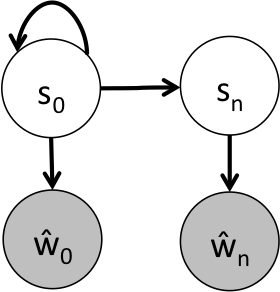
\includegraphics[width=0.25\textwidth]{MDPs_2.png}
\caption{MDP for two-steps RTB auction}
\label{fig:MDPs_2}
\end{figure}
In a two-steps auction, 
\begin{equation}
U(s) = \left( {\begin{array}{*{20}{c}}
{{k_{00}}}&{{k_{n0}}}
\end{array}} \right){\left[ {\left( {\begin{array}{*{20}{c}}
{{k_{00}}}&{{k_{n0}}}\\
{{k_{0n}}}&{{k_{nn}}}
\end{array}} \right) - \delta P\left( {\begin{array}{*{20}{c}}
{{k_{00}}}&{{k_{n0}}}\\
{{k_{0n}}}&{{k_{nn}}}
\end{array}} \right)} \right]^{ - 1}}\left( {\begin{array}{*{20}{c}}
0\\
{u({b_i},{\theta _i})}
\end{array}} \right)
\end{equation}
where the transition matrix $P$ is given by
\begin{equation}
P=\begin{bmatrix}
F_{0}(b_i) & 1-F_{0}(b_i)\\ 
0 & 0 
\end{bmatrix}
\end{equation}
It can be simplified as
\begin{equation}
U(s) = \frac{{{k_{00}}{k_{nn}} - {k_{0n}}{k_{n0}}}}{{\left| A \right|}}\left[ {\begin{array}{*{20}{c}}
1&{\delta (1 - {F_0}({b_i}))}
\end{array}} \right]\left( {\begin{array}{*{20}{c}}
0\\
{u({b_i},{\theta _i})}
\end{array}} \right)
\end{equation}
where $\left| A \right| = (1 - \delta {F_0}({b_i}))({k_{00}}{k_{nn}} - {k_{0n}}{k_{n0}})$. Thus, the total utility is equivalent to a closed form solution
\begin{equation}
\label{eq:keUs}
U(s) = \frac{{\delta (1 - {F_0}({b_i}))}}{{1 - \delta {F_0}({b_i})}}u({b_i},{\theta _i})
\end{equation}
and $u({b_i},{\theta _i})$ is given by Eq.~\ref{eq:utility}. Hence, the optimal bid will be
\begin{equation}
\label{eq:kernelbid}
b^{*}_{i}=\underset{b_i}\argmax \frac{{\delta (1 - {F_0}({b_i}))}}{{1 - \delta {F_0}({b_i})}}u({b_i},{\theta _i})
\end{equation}
Assume $f_0$ follows a uniform distribution varying from 0 to 1. Eq.~\ref{eq:keUs} is
\begin{equation}
\label{eq:kerneluni}
U(s) = \frac{{\delta (1 - {b_i})}}{{1 - \delta {b_i}}}({\theta _i}b_i^{N - 1} - \frac{{N - 1}}{N}b_i^N)
\end{equation}
and let the first-order differential equation of Eq.~\ref{eq:kerneluni} be zero 
\begin{equation}
\frac{{\partial U(s)}}{{\partial b_i}} = \frac{{\partial \frac{{\delta (1 - {b_i})}}{{1 - \delta {b_i}}}({\theta _i}b_i^{N - 1} - \frac{{N - 1}}{N}b_i^N)}}{{\partial b_i}} = 0
\end{equation}
If $b_i=0$, the first-order differential equation is positive. If $b_i=1$, it is negative. Meanwhile, if $b_i=\theta_i$, the first-order differential equation is also positive rather than zero. It implies that the optimal bid is at true value. The number letting differential equation become zero between true value $\theta_i$ and 1 gives the optimum value. This value is larger than true value in the beginning. 
Likewise, if the advertiser can know all the information after two bids, 
\begin{figure}[htbp]
\centering
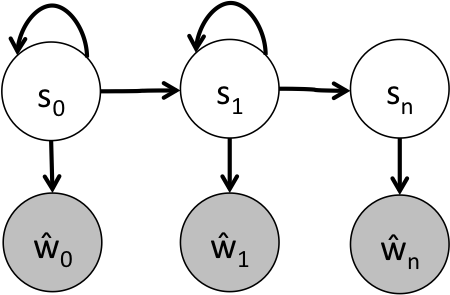
\includegraphics[width=0.4\textwidth]{MDPs_3.png}
\caption{MDP for three-steps RTB auction}
\label{fig:MDPs_3}
\end{figure}
In three-steps auction, the transition matrix is changed to
\begin{equation}
P=\begin{bmatrix}
F_{0}(b_i) & 1-F_{0}(b_i) & 0 \\ 
 0 & F_{1}(b_i) &1-F_{1}(b_i) \\ 
 0 & 0  & 0
\end{bmatrix}
\end{equation}
Thus, using the approximation method also can find an approximated solution similar as Eq.~\ref{eq:kernelbid}. Further, this process can be extended to finite steps. The update from $f_n$ to $f_{n+1}$ uses Greedy Product-Limit Algorithm with respect to Eq.~\ref{eq:PL}. 

The result of Kernelized Value Function Approximation can be treated as an analytic solution. We will make a comparison between this and the computational results from Q-Learning and Sarsa later.











